\section{Foundations}
\label{sec:foundation}

In the introduction section, different use cases for the definition of OCL constraints on different
models and meta-models have been depicted. As identified in \cite{demuthRGWS09}, OCL evaluation
always requires three meta levels of the \emph{MOF Four Layer Metadata Architecture} \cite{spec:MOF1-4}. OCL can 
be considered an extension of a modelling language. Thus, its
abstract syntax must extend a meta-model that defines types, navigable properties, and operations
(cf. Fig.~\ref{fig:genericlayers}, (a), Mn+1 layer). This extension allows the definition of
OCL constraints on models of this meta-model (Mn layer). 
During the evaluation of these constraints, an OCL interpreter has to query model
instance elements for their properties or invoke operations on them (Mn-1 layer). 

	\begin{figure}[t]
			\centering
				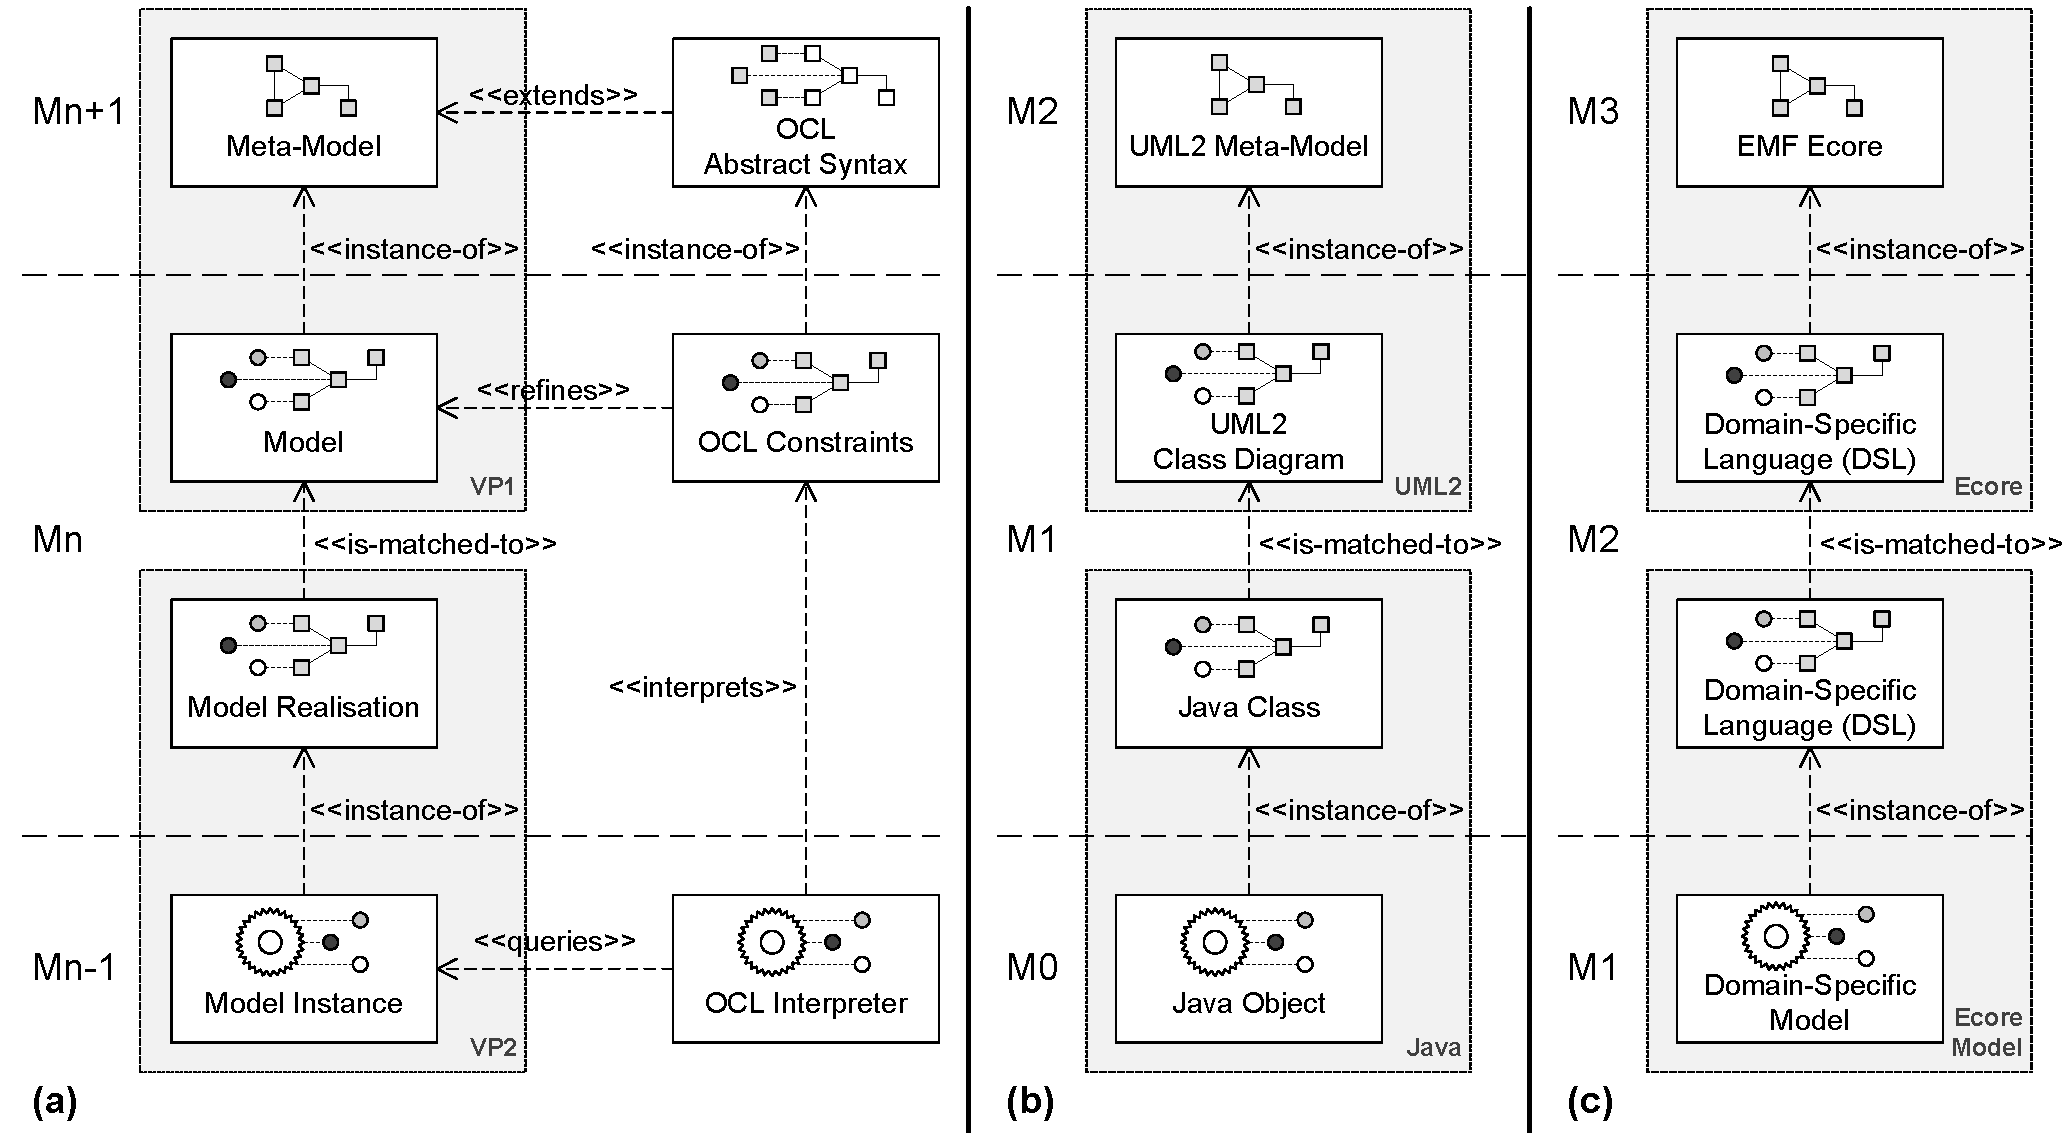
\includegraphics[width=1.00\textwidth]{figures/genericlayers.pdf}
			\caption{The Generic Three Layer Architecture}
			\label{fig:genericlayers}
		\end{figure}
	%\note{Fig 1. add headings to subfigures: a) Variation points in OCL Application	b) Applciation of OCL in UML modeling c) Application of OCL in Ecore
	%metamodeling } 

Model instances can be realised in
a different \emph{Technological Space}~\cite{kurtev2002technological} than their model. Then, there are two model
representations at the Mn layer: the constrained model and a \emph{Model Realisation} that can be obtained by a
\emph{Reflection} \cite{smith1982procedural} mechanism of the 
model instance. Thus, there has to be a matching of the model realisation to the constrained model.

Instances of this \emph{Generic Three Layer Architecture} are shown in Fig.~\ref{fig:genericlayers} 
(b) and (c). The first example illustrates the use of a UML class diagram constrained with business
rules for which model instance
elements are Java objects. At the layer M1 a technical space bridge can be observed, as the Java
classes correspond to the UML model. The second example depicts the usage of OCL for Well-Formedness
Rules (WFRs). Here, the model is a domain-specific language modelled in Ecore (M2) for which WFRs are
evaluated on domain-specific models (M1). In this case, the model and its realisation are identical.

With the generic three layer architecture it is possible to combine various models and instances for
constraint interpretation independently as depicted as a feature model in Fig.~\ref{fig:features}. 
The feature selection has to ensure that model
instances are located exactly one meta-layer below their model. In the feature model two variation
points regarding OCL interpretation can be identified: constrained models (VP1) as well as
model instances (VP2) can vary.

	\begin{figure}[t]
			\centering
		  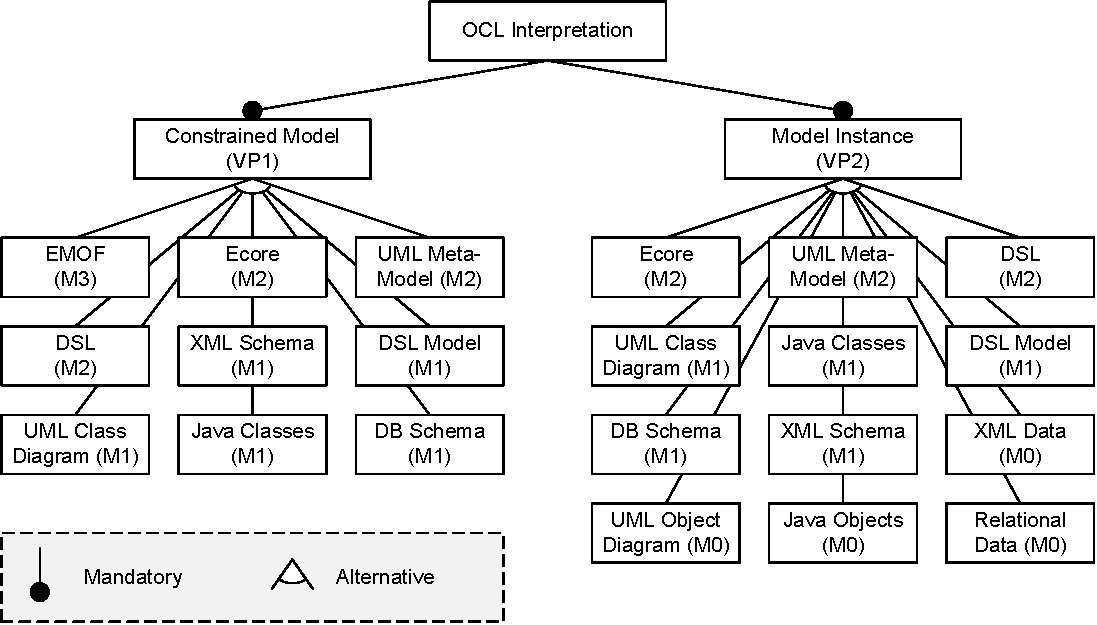
\includegraphics[width=1.00\textwidth]{figures/features.pdf}
			\caption{Features of OCL Interpretation}
			\label{fig:features}
	\end{figure}
	
In order to define constraints on different models, most OCL tools existing today, support VP1 
\cite{WWW:MDT,akehurst2003ocl,WWW:dresdenOCL,kolovos2008detecting}. Yet, those tools do not address
VP2 as their supported models require specific instances (typically located in the same technological
space). As presented in this paper, this tight coupling is not necessary and a reimplementation of
OCL interpreters for different technological spaces can be avoided.
We propose an implementation of the generic three layer architecture to address this problem.

	
	
	
	

% The \textit{Generic Three Layer Meta data Architecture}. (a): Each OCL constraint requires a meta-model defining a model on which OCL constraints are specified. The 
%			constraints are evaluated on a model instance that instantiates the constrained model. 
%			The generic architecture can be parametrized at two different variation points. Different
%			models and their meta-models can be bound to VP1, different model instances can be bound
%			to VP2.	(b): UML-Example for layers M2, M1 and M0. VP1 is bound to the UML meta-model (MOF), 
%			VP2 is bound to Java. (c): EMF-Example for layers M3, M2 and M1. VP1 is bound to EMF Ecore,
%			VP2 is bound to Ecore-based models.
%
%	To differentiate between meta-models, models and runtime objects, the OMG introduced 
%	the \textit{MOF Four Layer Metadata Architecture}, that locates the meta-model, 
%	model, and the model's instances at the layers \textit{M2}, \textit{M1} and \textit{M0}. 
%	\note{Is that important to understand the paper?; Michael: agreed, just refer to it, but leave explaination}{Each language at layer
%	\textit{Mn} is described in terms of a language resided at layer \textit{Mn-1}. Meta-meta-models 
%	that are located at the layer \textit{M3} 
%	can describe themselves reflexively.}
%	
%	Fig.~\ref{fig:genericlayers} depicts the \textit{Generic Three Layer
%	Meta-Data Architecture} aligning OCL constraints with the MOF layers.
%	\remove{As all
%	models can be located in this layer architecture, OCL can be located there as
%	well.} OCL constraints are a model and can be described using their abstract
%	syntax, i.e., the OCL meta-model. They are evaluated for runtime objects at the 
%	model instance layer. 
%	%\remove{Thus, three layers must be known by the OCL tool
%	%to define and evaluate the constraints. This notion leads to the 
%	%Generic Three Layer Meta-Data Architecture demuthRGWS09} that 
%	%allows to define an OCL tool independently of specific layers. As can be seen
%	%in Figure \ref{fig:genericlayers} the OCL model (all constraints) enriches
%	%another model.} 
%	In order to \change{navigate through the  model or to call
%	operations on}{define constraints on models OCL needs to navigate on} model
%	elements. To bind OCL constraints on the navigation structure in
%	the model they are defined on, the abstract syntax of OCL
%	\note{this is true for UML, but sounds quite technical}{extends} the model's
%	meta-model.
%	%OCL can be used to define well-formedness rules, i.e., constraints on meta-models (M2) that are evaluated at the model level (M1), or business rules, i.e., constraints defined on models (M1) that are evaluated for runtime objects at the model instance layer (M0).
%	
%	\note{we need to incorporate the motivation for implementation language
%	variation here. Reviewers need to understand the problem to understand our
%	solution.}
%
%
%	\note{This section does not clarify the contribution of THIS paper. We should
%	sell the instance adaptation as a improvement of previous DresdenOCL versions
%
%	
%	}
%
%	{The architecture of Dresden OCL2 for Eclipse was developed in respect to the 
%	generic three layer meta-data architecture. In order to reuse the developed 
%	OCL tools, DresdenOCL does not directly accesses models or model instance objects. 
%	Instead, these are hidden behind a common set of interfaces that delegate to 
%	their adaptee. The adaptation of models and model instance objects is presented 
%	in the following.}


